\documentclass[xcolor=usenames,xcolor=svgnames,table,slidestop,compress,mathserif]{beamer}
%\documentclass{beamer}
\usepackage[utf8x]{inputenc}
%\usepackage{pgf}
\usepackage{graphicx}
\usepackage[usenames,svgnames]{xcolor}

\usepackage{amsmath}
\usepackage{amssymb}
\usepackage{floatflt}
\usepackage{booktabs} %for nice tables
\usepackage{multirow}
\usepackage{qtree}
\usepackage{subfigure}
\usepackage{textcomp} %for uparrow
%\usepackage{tweaklist}
\usepackage{fancybox}
%\usepackage{verbatim}
\usepackage{subfigure}
\newcommand{\rd}[0]{\ensuremath{\mathcal{R}}}
\newcommand{\rds}[0]{\ensuremath{\mathcal{R}} }
\newcommand{\adv}[0]{\ensuremath{\mathcal{A}} }

\newcommand{\outc}[2] {\overline{c_{#1}}\langle #2 \rangle}
\newcommand{\realeq}{\stackrel{\Delta}{=}}
\newcommand{\ki}[0]{\texttt{<}}
\newcommand{\be}[0]{\texttt{>}}
\usepackage[algoruled, linesnumbered, lined]{algorithm2e} %algorithms

\usepackage{beamerthemesplit}
%\usetheme{Berlin}
%\usetheme{Singapore}
%\useoutertheme{miniframes}

\usetheme{Madrid}
%\usetheme{Antibes}

%\usecolortheme{lily}
\usecolortheme{seahorse}

%\beamertemplateshadingbackground{blue!5}{yellow!10}
\beamertemplateshadingbackground{blue!6}{white}
\beamertemplateballitem

\newcommand{\comb}[2]{\ensuremath{\left(\begin{array}{c} #1\\ #2 \end{array} \right)}}

\title[Grain of Salt]{Grain of Salt
}
\subtitle{An Automated Way to Test
Stream Ciphers through SAT Solvers\\\tiny Presentation at Tools for Cryptanalysis}
\author[Mate Soos]{\sc Mate Soos\footnote{The author was supported by the RFID-AP ANR Project, project number
\texttt{ANR-07-SESU-009}}}
\institute{UPMC LIP6, PLANETE team INRIA, SALSA team INRIA}

\date{23rd June 2010}





\AtBeginSection[]
{
   \begin{frame}
       \frametitle{Outline}
       \tableofcontents[currentsection]
   \end{frame}
}

%\newcommand{\outc}[2] {\overline{c_{#1}}\langle #2 \rangle}
%\newcommand{\realeq}{\stackrel{\Delta}{=}}
%\newcommand{\ki}[0]{\texttt{<}}
%\newcommand{\be}[0]{\texttt{>}}

\begin{document}

\begin{frame}
  \titlepage
\end{frame}

\frame{
\frametitle{Table of Contents}
\setcounter{tocdepth}{1}
\tableofcontents
}
\setcounter{tocdepth}{2}

\section{Context}

%\subsection{Motivations and goals}
\frame
{
\frametitle{Motivations and goals}
\begin{beamerboxesrounded}[shadow=true]{Motivations}
   \begin{itemize}
    \item Stream ciphers may be broken using SAT solving tools
    \item Analysis of stream ciphers is possible using SAT solvers
   \end{itemize}
\end{beamerboxesrounded}

\bigskip
\begin{beamerboxesrounded}[shadow=true]{Goals}
   \begin{itemize}
    \item Describe different methods to translate shift register-based stream ciphers to SAT problems
    \item Demonstrate a tool that can help in this process
   \end{itemize}
\end{beamerboxesrounded}
}

\subsection{SAT solvers}
\frame
{
\frametitle{What is a SAT solver}
\begin{beamerboxesrounded}[shadow=true]{Solves a problem in CNF}
CNF is an ``\texttt{and} of \texttt{or}-s''
\begin{displaymath}
   (x_1 \vee \neg x_3)  \quad \wedge \quad (\neg x_2 \vee x_3) \quad \wedge \quad (x_1 \vee x_2)
\end{displaymath}
\end{beamerboxesrounded}

\smallskip
\begin{beamerboxesrounded}[shadow=true]{Uses DPLL($\varphi$) algorithm}
  \begin{enumerate}
  \small
   \item If formula $\varphi$ is trivial, return SAT/UNSAT
   \item ret = DPLL($\varphi$ with $v$ $\leftarrow$ \texttt{true})
   \item if ret == SAT, return SAT
   \item ret = DPLL($\varphi$ with $v$ $\leftarrow$ \texttt{false})
   \item if ret == SAT, return SAT
   \item return UNSAT
 \end{enumerate}
 \end{beamerboxesrounded}
}

\frame
{
\frametitle{Search tree}
\begin{columns}[T]
  \begin{column}{8.5cm}
  \begin{beamerboxesrounded}[shadow=true]{Example search tree}

  \begin{figure}[ht]
  \begin{center}
  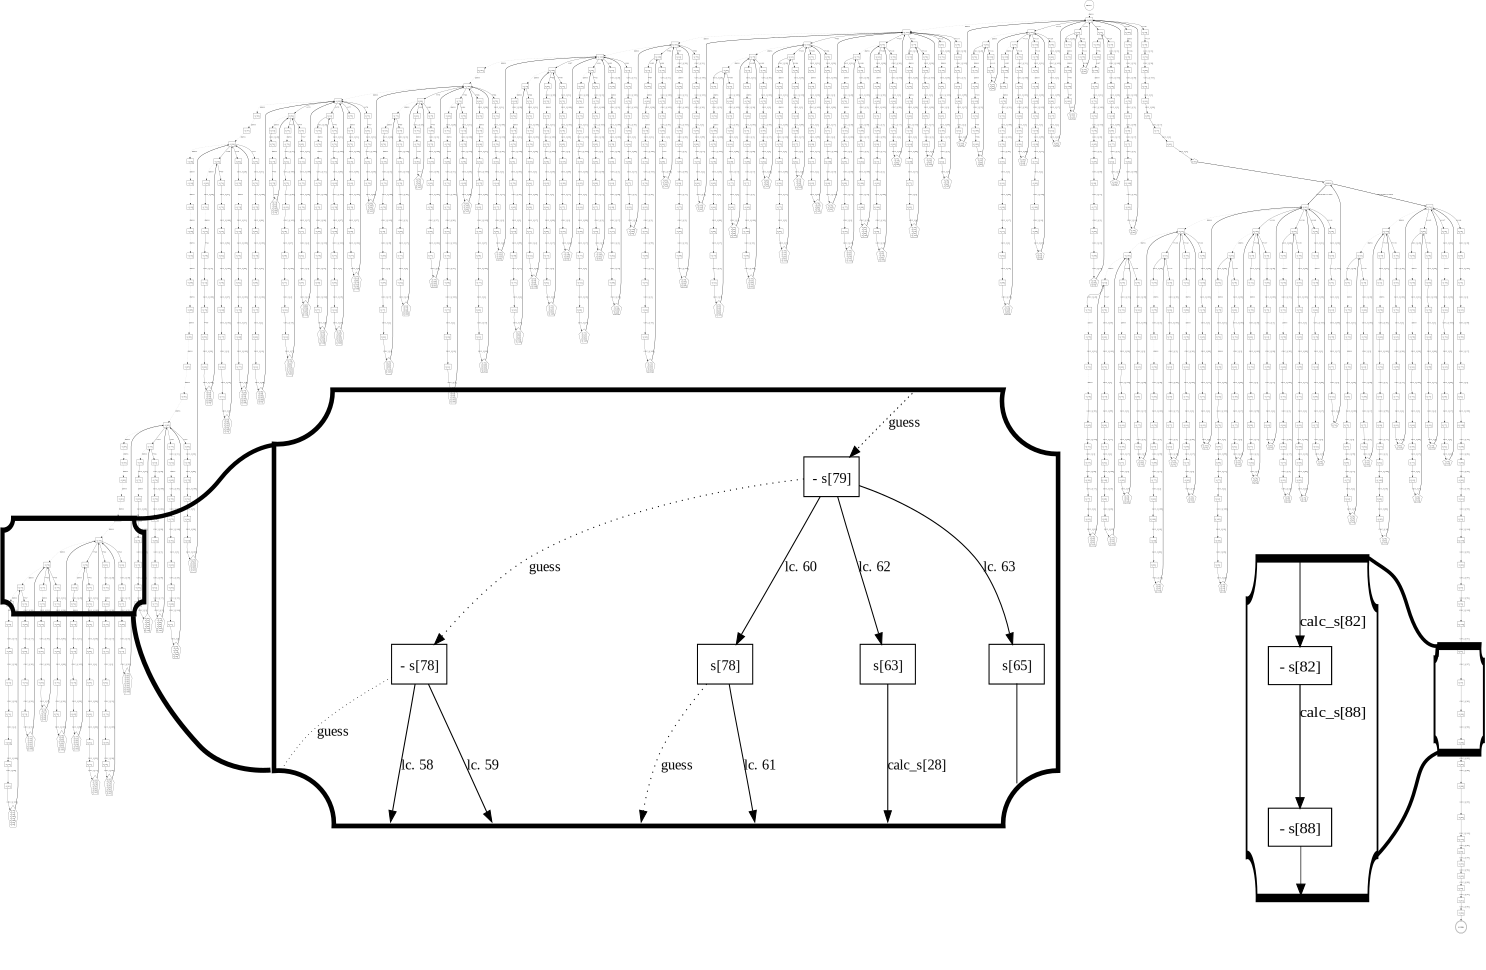
\includegraphics[width=8.6cm]{search_graph/search_graph2}
  \end{center}
  \end{figure}
  
  \end{beamerboxesrounded}
  \end{column}
  
  \begin{column}{3cm}
   \begin{beamerboxesrounded}[shadow=true]{Visualised}
   \tiny
   %\renewcommand{\itemhook}{\setlength{\topsep}{0pt} \setlength{\itemsep}{0pt}}
    \begin{itemize}
     \item Guesses
     \item Propagations
     \item Generated learnt clauses
     \item Clause group causing the propagation
    \end{itemize}
   \end{beamerboxesrounded}
   
   \bigskip
   \begin{beamerboxesrounded}[shadow=true]{Calculated stats}
   \tiny
    \begin{itemize}
     \item Average depth
     \item Most conflicted clauses
     \item No. of guess/branch
     \item Most guessed vars
     \item Most propagated vars
    \end{itemize}
   \end{beamerboxesrounded}
 
  \end{column}
  
\end{columns}
}

% \frame
% {\frametitle{SAT solver internals}
% \begin{beamerboxesrounded}[shadow=true]{Conflict clauses}
%    \begin{itemize}
%     \item Generated when current assignment doesn't satisfy a clause
%     \item Collection of information leading to conflict
%     \item Used to avoid similar wrong parts of the tree next time
%    \end{itemize}
% \end{beamerboxesrounded}
% 
% \bigskip
% \begin{beamerboxesrounded}[shadow=true]{Most important parts}
%    \begin{itemize}
%     \item Lazy data structures
%     \item Learning (and forgetting)
%     \item How to pick a variable
%     \item When to restart
%    \end{itemize}
% \end{beamerboxesrounded}
% }

\subsection{Stream ciphers}

\frame
{
\frametitle{Stream ciphers}
\begin{beamerboxesrounded}[shadow=true]{Shift register-based stream ciphers}
\begin{itemize}
 \item Use a set of \emph{shift registers}
 \item Shift registers' \emph{feedback function} is either linear or non-linear
 \item Uses a \emph{filter function} to generate 1 secret bit from the state
 \item Working: clock-filter-clock-filter\ldots feedback-filter-feedback-filter\ldots
\end{itemize}
\end{beamerboxesrounded}

\begin{beamerboxesrounded}[shadow=true]{Example cipher}
\begin{figure}
\centering
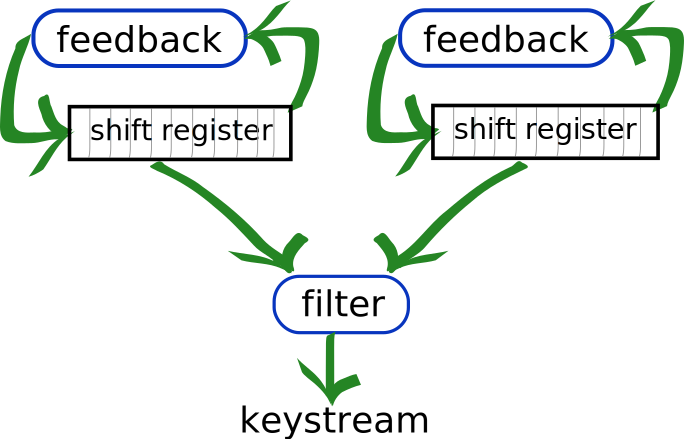
\includegraphics[height=4cm]{stream_cipher/stream_cipher}
\end{figure}
\end{beamerboxesrounded}
}

\section{Translating shift register-based stream ciphers to SAT problems}

\frame
{\frametitle{Translating shift register-based stream ciphers to CNF}
\begin{beamerboxesrounded}[shadow=true]{Unwinding time}
\begin{itemize}
 \item SAT solvers don't understand the notion of ``time''
 \item We must present the problem as if no timing was involved
 \item To make unwinding simple, regular clocking is needed
\end{itemize}
\end{beamerboxesrounded}

\smallskip

\begin{beamerboxesrounded}[shadow=true]{Describe feedback and filter functions}
\begin{itemize}
 \item Translate ANF (Algebraic Normal Form) to CNF
 \item Either through XORs and Monomials
 \item Or through direct translation using Karnaugh maps
\end{itemize}
\end{beamerboxesrounded}

\smallskip

\begin{beamerboxesrounded}[shadow=true]{Give help bits to aid solving}
\begin{itemize}
 \item Select and fix shift register states: guess-and-determine
 \item Select shift register states randomly, fix randomly, and solve for random problems
\end{itemize}
\end{beamerboxesrounded}
}

\subsection{Unwinding time}

\frame
{\frametitle{Unwinding time}
\begin{beamerboxesrounded}[shadow=true]{Why unwind?}
\begin{itemize}
 \item CNF cannot handle the notion of ``time''
 \item Must present all shift register states in the CNF at once
 \item No irregular clockings
\end{itemize}
\end{beamerboxesrounded}

\bigskip

\begin{beamerboxesrounded}[shadow=true]{Example}
\begin{itemize}
 \item Crypto1 state: 48 bits
 \item We have observed 56 bits of output
 \item We need to clock 56 times
 
 \smallskip
 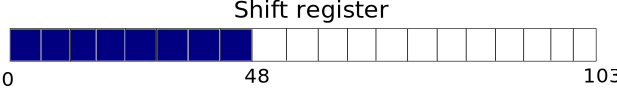
\includegraphics[width=9cm]{shifting/unwind}
\end{itemize}
\end{beamerboxesrounded}
}

\frame
{\frametitle{Unwinding the time}
\begin{beamerboxesrounded}[shadow=true]{Base-shifting}
\begin{itemize}
\item If the feedback functions are reversible, we can start in the middle
\item Usually best to shift to the middle:

\smallskip
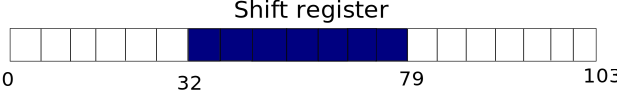
\includegraphics[width=9cm]{shifting/shifting}

\item The total depth of the search is then halved
\end{itemize}
\end{beamerboxesrounded}

\bigskip

\begin{beamerboxesrounded}[shadow=true]{Grain of Salt}
\begin{itemize}
\item \texttt{./grainofsalt --outputs 56 --crypto crypto1\\
                            \qquad \qquad \qquad \quad --base-shift 32}
\item \texttt{./grainofsalt --outputs 160 --crypto grain\\
                            \qquad \qquad \qquad \quad --base-shift 80,80}
\end{itemize}
\end{beamerboxesrounded}
}

\subsection{Describing feedback and filter functions}
\frame
{\frametitle{Describing feedback and filter functions}
\begin{beamerboxesrounded}[shadow=true]{ANF$\rightarrow$CNF}
\begin{itemize}
 \item ANF (Algebraic Normal Form): $a = bc \oplus b \oplus c$
 \item Must be converted to CNF: $x \vee y = \texttt{true}$
 \item[1] Assign each higher degree monomial an internal variable
 \item[2] Describe the XOR as CNF
\end{itemize}
\end{beamerboxesrounded}

\begin{beamerboxesrounded}[shadow=true]{Extended monomials}
\begin{itemize}
 \item CNF does not limit terms to be non-negated as ANF does
 \item $bc\oplus b \oplus c= b(c+1) \oplus c= (b+1)(c+1)\oplus 1 = \neg b \neg c \oplus 1$
 \item Default in \texttt{grainofsalt}, can be disabled with \texttt{--noextmonomials}
%  \begin{align}
%  \neg b \vee \neg c \vee i_1\\
%  b \vee \neg i_1\\
%  c \vee \neg i_1\\
%  \end{align}
\end{itemize}
\end{beamerboxesrounded}

\begin{beamerboxesrounded}[shadow=true]{Karnaugh maps}
\begin{itemize}
 \item Uses Karnaugh maps to map functions to CNF
 \item Does not need internal variables
 \item May generate substantially smaller function descriptions
\end{itemize}

\end{beamerboxesrounded}

% \begin{beamerboxesrounded}[shadow=true]{XOR$\rightarrow$CNF}
% \begin{itemize}
%  \item $i_i \oplus b \oplus c = true$ represented as:
% \begin{align}
%  i_1 \vee b \vee c\\
%  \neg i_1 \vee \neg b \vee c\\
%  \neg i_1 \vee b \vee \neg c\\
%  i_1 \vee \neg b \vee \neg c\\
%  \end{align}
%  \item if XOR is too large, internal it must be cut into pieces
% \end{itemize}
% \end{beamerboxesrounded}
}

\begin{frame}[fragile]
\frametitle{Describing feedback and filter functions}

\begin{beamerboxesrounded}[shadow=true]{Function descriptions in \texttt{grainofsalt}}
File \texttt{grain/functions/sr0/feedback.txt}
{\small\begin{verbatim}
sr1-62
sr1-51
sr1-38
sr1-23
sr1-13
sr1-0
\end{verbatim}}
Defines feedback function:
$s_{i+80} = s_{i+62} + s_{i+51} + s_{i+38} + s_{i+23} + s_{i+13} + s_i$
\end{beamerboxesrounded}

\begin{beamerboxesrounded}[shadow=true]{Arbitrary functions}
\begin{itemize}
 \item Arbitrary functions can be defined and used in other functions
 \item Dependency graph is built from output bits, only used functions are generated in CNF
 \item Allows to efficiently map ciphers built from functional blocks
\end{itemize}
\end{beamerboxesrounded}
\end{frame}

\frame[c]
{\frametitle{Describing feedback and filter functions}
\begin{figure}
\centering
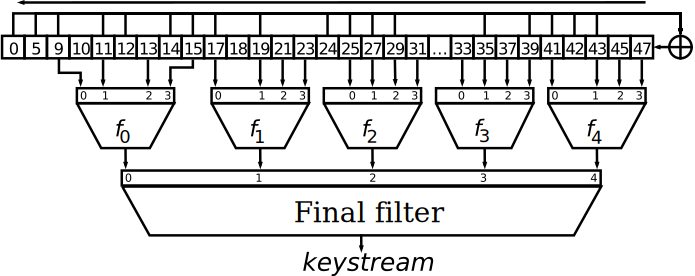
\includegraphics[height=4.5cm]{crypto1_2.pdf}
\caption{Crypto-1 cipher filter function diagram}
\end{figure}
}


\subsection{Help bits}

\frame
{\frametitle{Help bits}
\begin{beamerboxesrounded}[shadow=true]{Why?}
\begin{itemize}
 \item Usually the generated problem is too slow to solve
 \item Except when breaking Crypto-1 (London travel card) --- 40sec. approx
 \item[1] Give bits at fixed positions, multiply
 \item[2] Give bits at random positions, extrapolate
\end{itemize}
\end{beamerboxesrounded}

\bigskip

\begin{beamerboxesrounded}[shadow=true]{Given information use}
\begin{itemize}
\item Recursively propagated at the ANF level
\item Monomials are replaced with their constant equivalents
\item Monomials are replaced with their monomial equivalents
\item To disable: \texttt{--nopropagate}
\end{itemize}
\end{beamerboxesrounded}
}

\frame
{\frametitle{Help bits}
\begin{beamerboxesrounded}[shadow=true]{Fixed help bits}
\begin{itemize}
\item Difficult to know which combination of variables will be fastest
\item Automated, randomised (Monte Carlo) greedy algorithm
\item Sets all bits, tests difficulty based on generated CNF size
\item Average smallest size wins
\item To generate: \texttt{--genDeterBits N} To use: \texttt{--deterBits N}
\end{itemize}
\end{beamerboxesrounded}

\smallskip

\begin{beamerboxesrounded}[shadow=true]{Probabilistic help bits}
\begin{itemize}
\item Fix $n$ randomly picked vars randomly, measure time
\item Do above step (\emph{everything} random) many times and average
\item Do above steps for $n-1,n-2\ldots$ until possible
\item Plot graph --- if done well, it is perfectly exponential
\item But exponential factor $\ll 2$
\item To use: \texttt{--probBits N}
\end{itemize}
\end{beamerboxesrounded}
}

\subsection{Overview}
\frame{
\frametitle{Overview}
\begin{beamerboxesrounded}[shadow=true]{Flow diagram}
\begin{figure}
\centering
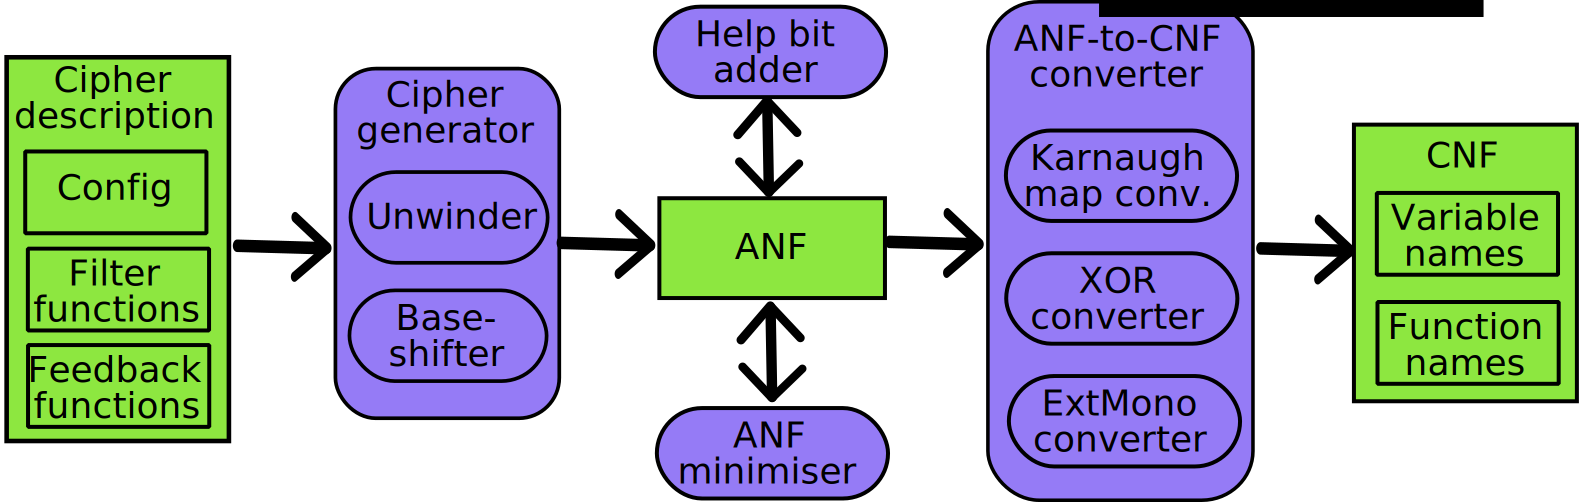
\includegraphics[width=12cm]{diagram/drawing}
%\caption{Valami}
\end{figure}
\end{beamerboxesrounded}

\begin{beamerboxesrounded}[shadow=true]{Example usage}
\begin{itemize}
 \item \texttt{./grainofsalt --crypto grain --outputs 100 --genDeterBits 60}
 \item \texttt{./grainofsalt --crypto grain --outputs 100 --stats --cnfDir generatedCNFs --num 100 --deterBits 55}
 %\item \texttt{./grainofsalt --crypto trivium --outputs 180 --init no  --base-shift 60.60,60 --probBits 100}
\end{itemize}
\end{beamerboxesrounded}
}

\section{Conclusions}
\frame[c]
{\frametitle{Conclusions}

\begin{beamerboxesrounded}[shadow=true]{Concluding remarks}
\begin{itemize}
 \item \texttt{grainofsalt} gives an integrated platform to conduct experiments with SAT solvers on shift register-based stream ciphers
 \item It is GPL, with open GIT repository, well-documented, and extensible
 \item \url{http://gitorious.com/grainofsalt/}
\end{itemize}
\end{beamerboxesrounded}

\bigskip
\begin{beamerboxesrounded}[shadow=true]{Future work}
\begin{itemize}
 \item Add more ciphers --- they are very simple to describe
 \item Add more functionality --- non-shift register based ciphers
 \item Could be integrated into \texttt{sage} partially/fully
\end{itemize}
\end{beamerboxesrounded}

}

\frame[c]
{
   \begin{figure}
   \begin{center}
 {\huge
  Thank you for your time}
 \bigskip

\bigskip

\Large
Any questions?
   \end{center}
   \end{figure}
}


\end{document}